\documentclass[]{tufte-handout}

% ams
\usepackage{amssymb,amsmath}

\usepackage{ifxetex,ifluatex}
\usepackage{fixltx2e} % provides \textsubscript
\ifnum 0\ifxetex 1\fi\ifluatex 1\fi=0 % if pdftex
  \usepackage[T1]{fontenc}
  \usepackage[utf8]{inputenc}
\else % if luatex or xelatex
  \makeatletter
  \@ifpackageloaded{fontspec}{}{\usepackage{fontspec}}
  \makeatother
  \defaultfontfeatures{Ligatures=TeX,Scale=MatchLowercase}
  \makeatletter
  \@ifpackageloaded{soul}{
     \renewcommand\allcapsspacing[1]{{\addfontfeature{LetterSpace=15}#1}}
     \renewcommand\smallcapsspacing[1]{{\addfontfeature{LetterSpace=10}#1}}
   }{}
  \makeatother
\fi

% graphix
\usepackage{graphicx}
\setkeys{Gin}{width=\linewidth,totalheight=\textheight,keepaspectratio}

% booktabs
\usepackage{booktabs}

% url
\usepackage{url}

% hyperref
\usepackage{hyperref}

% units.
\usepackage{units}

\usepackage{etoolbox}
\makeatletter
\patchcmd{\@caption}
  {\noindent\csname fnum@#1\endcsname: \ignorespaces}
  {}
  {}{}
\makeatother



\setcounter{secnumdepth}{-1}

% citations
\usepackage{natbib}
\bibliographystyle{plainnat}

% pandoc syntax highlighting

% longtable

% multiplecol
\usepackage{multicol}

% strikeout
\usepackage[normalem]{ulem}

% morefloats
\usepackage{morefloats}
\geometry{bottom=1.5cm}

% tightlist macro required by pandoc >= 1.14
\providecommand{\tightlist}{%
  \setlength{\itemsep}{0pt}\setlength{\parskip}{0pt}}

% title / author / date
\title{Disputation: Epistemische Überzeugungen \mbox{Lehramtsstudierender}}
\date{Samuel Merk, Juli 2016}

\parindent0pt

\begin{document}

\maketitle




\section{Einführung}\label{einfuhrung}

\begin{marginfigure}
Folien: \url{http://46.101.230.125:3838/Disputation}; Quellcode:
\url{https://github.com/sammerk/Disputation}
\end{marginfigure}

Der Begriff \textbf{Epistemologie} stellt ein modernes Kompositum aus
\emph{Episteme (= Erkenntnis, Wissen, Wissenschaft)} und \emph{Logos (=
Wissenschaft, Lehre)}\footnote{Meidl, C.N. (2009).
  \emph{Wissenschafts- theorien für SozialforscherInnen.} Wien: Böhlau.}
dar. \textbf{Epistemische Überzeugungen} werden in der Literatur als
Überzeugungen definiert, welche die Natur und Genese von Wissen
betreffen und typischerweise die Aspekte \emph{Quelle},
\emph{Rechtfertigung}, \emph{Struktur} und \emph{Komplexität}
beinhalten\footnote{Bråten, I. (2010). Personal Epistemology in
  Education: Concepts, Issues, and Implications. In: P. Peterson, E.
  Baker \& B. McGaw, (Hrsg.), \emph{International Encyclopedia of
  Education}, S. 211--217. Oxford: Elsevier.}.

\subsection{Begriffliche Vielfalt}\label{begriffliche-vielfalt}

Der in ersten Forschungsarbeiten verwendete Begriff ``epistemologi- sche
Überzeugungen'' unterliegt der Kritik, Überzeugungen bzgl. der
Wissenschaftstheorie zu definieren, wohingegen eigentlich Überzeugungen
gemeint sind, die Entitäten betreffen, welche auch in der
Wissenschaftstheorie vorkommen, aber nicht wissenschaftstheoretischer
Natur sind. Heute liegt eine Vielzahl an Begrifflichkeiten vor, die
auf jeweils unterschiedlich akzentuierten Konzeptualisierungen basieren.

\begin{marginfigure}
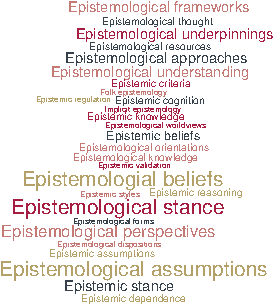
\includegraphics{Handout_files/figure-latex/fig-margin1-1} 
\caption{\noindent{Begrifflichkeiten nach Greene et al., (2016). Textgröße proportional zu Suchtrefferhäufigkeiten in GoogleScholar.}}
\label{fig:fig-margin1}
\end{marginfigure}
%\begin{marginfigure}
%Begrifflichkeiten nach Greene et al., (2016). Textgröße proportional zu Suchtrefferhäufigkeiten in GoogleScholar.
%\end{marginfigure}


\subsection{Systematisierung und Kritik gängiger
Konzeptualisierungen}\label{systematisierung-und-kritik-gangiger-konzeptualisierungen}

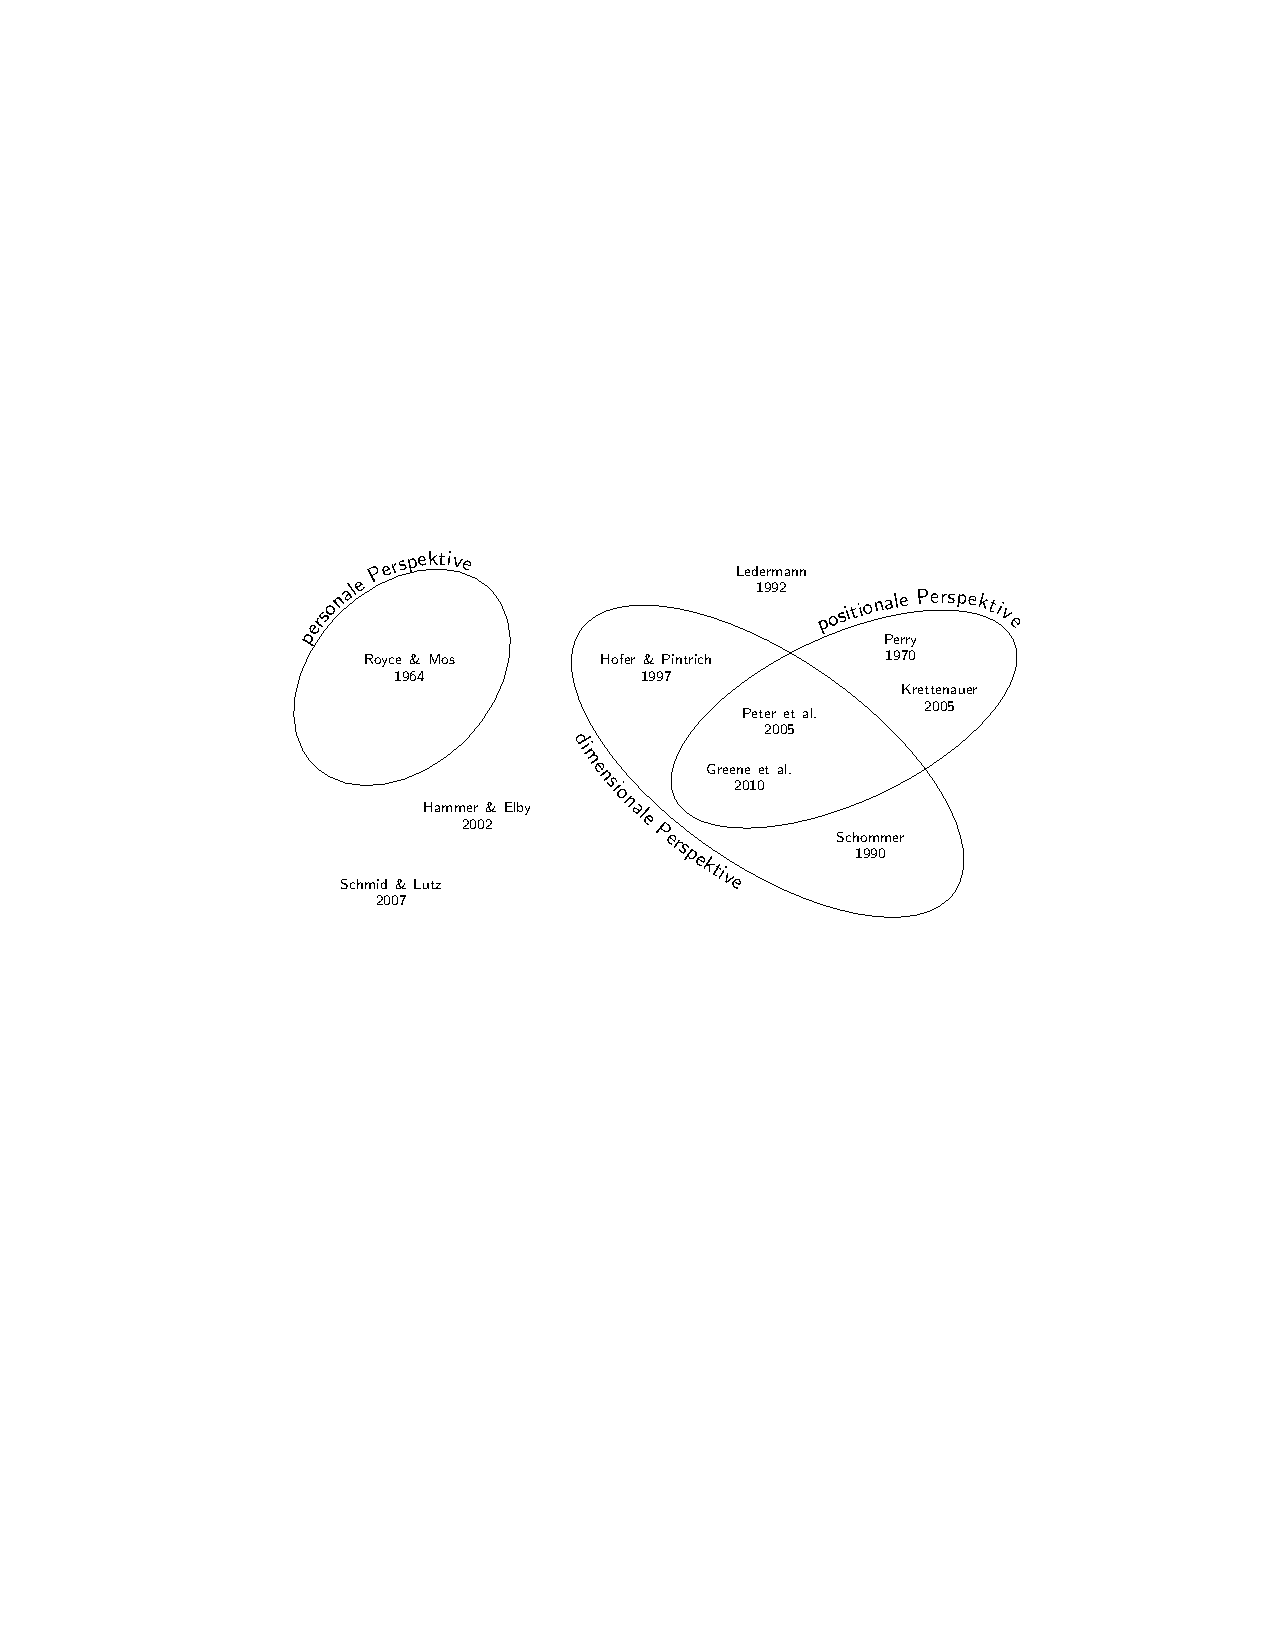
\includegraphics{../Img/Topologie.pdf} Als Hauptproblem der
Entwicklungsperspektive werden die starken Annahmen einer
eindimensionalen, sequentiellen Entwicklung in diskreten Stufen gesehen
(Konstruktvalidität), die empirisch nicht bestätigt werden können und
zudem abweichend von den Annahmen operationalisiert werden\footnote{Hofer,
  B. K., \& Pintrich, P. R. (1997). The Development of Epistemological
  Theories: Beliefs About Knowledge and Knowing and Their Relation to
  Learning. \emph{Review of Educational Research}, 67(1), 88--140.}. Die
Konstruktvalidität der dimensionalen Perspektive wird insbesondere durch
eine Interpretation der Dimensionen als ``naiv-sophistiziert Kontinuen''
geschwächt\footnote{Elby, A., \& Hammer, D. (2001). On the substance of
  a sophisticated epistemology. \emph{Science Education}, 85(5),
  554--567.}.
\pagebreak
\section{Synopse zentraler Befunde}\label{synopse-zentraler-befunde}

\begin{marginfigure}
\textbf{Modellierungsbeispiel:}
\[Rel_{ij} = \beta_{0j} + \beta_{1} \cdot  I^{Thema_1}_{ij} + ... + e_{ij}\]
\[\beta_{0j} = \gamma_{0} + \gamma_{1} \cdot Rel^{global}_{j} + u_{j}\]
Wobei i und j Indices für Thema und Person darstellen, Rel =
Relativismus, I = Kontrastkodierte Indikatorvariable, u bzw. e =
Residuen
\end{marginfigure}

\subsection{Epistemische Überzeugungen sind dualer
Natur}\label{epistemische-uberzeugungen-sind-dualer-natur}

Inwiefern sich epistemologische Unterschiede akademischer Domänen in
epistemischen Überzeugungen niederschlagen, ist für Lehramts-
studierende in besonderem Maße interessant, da diese vergleichs- weise
viele Domänen kennenlernen und ihre Curricula vergleichs- weise wenig
erkenntnistheoretische und methodische Inhalte vorsehen. Bei
gegenstandsspezifischer und globaler Erfassung sowie simultaner
Mehrebenen-Modellierungen von within- und between-person Varianz konnte
mehrfach Evidenz für die Hypothese einer \textbf{dualen Natur}
epistemischer Überzeugungen Lehramtsstudierender gefunden werden. Dabei
zeigte sich, dass between-person Effekte der \textbf{Domänen}, der
\textbf{Quelle}, des \textbf{Kontextes} etc. weit weniger stark sind,
als die within-person Differenzen über bildungswissenschaftliche
Gegenstände hinweg.

\begin{marginfigure}
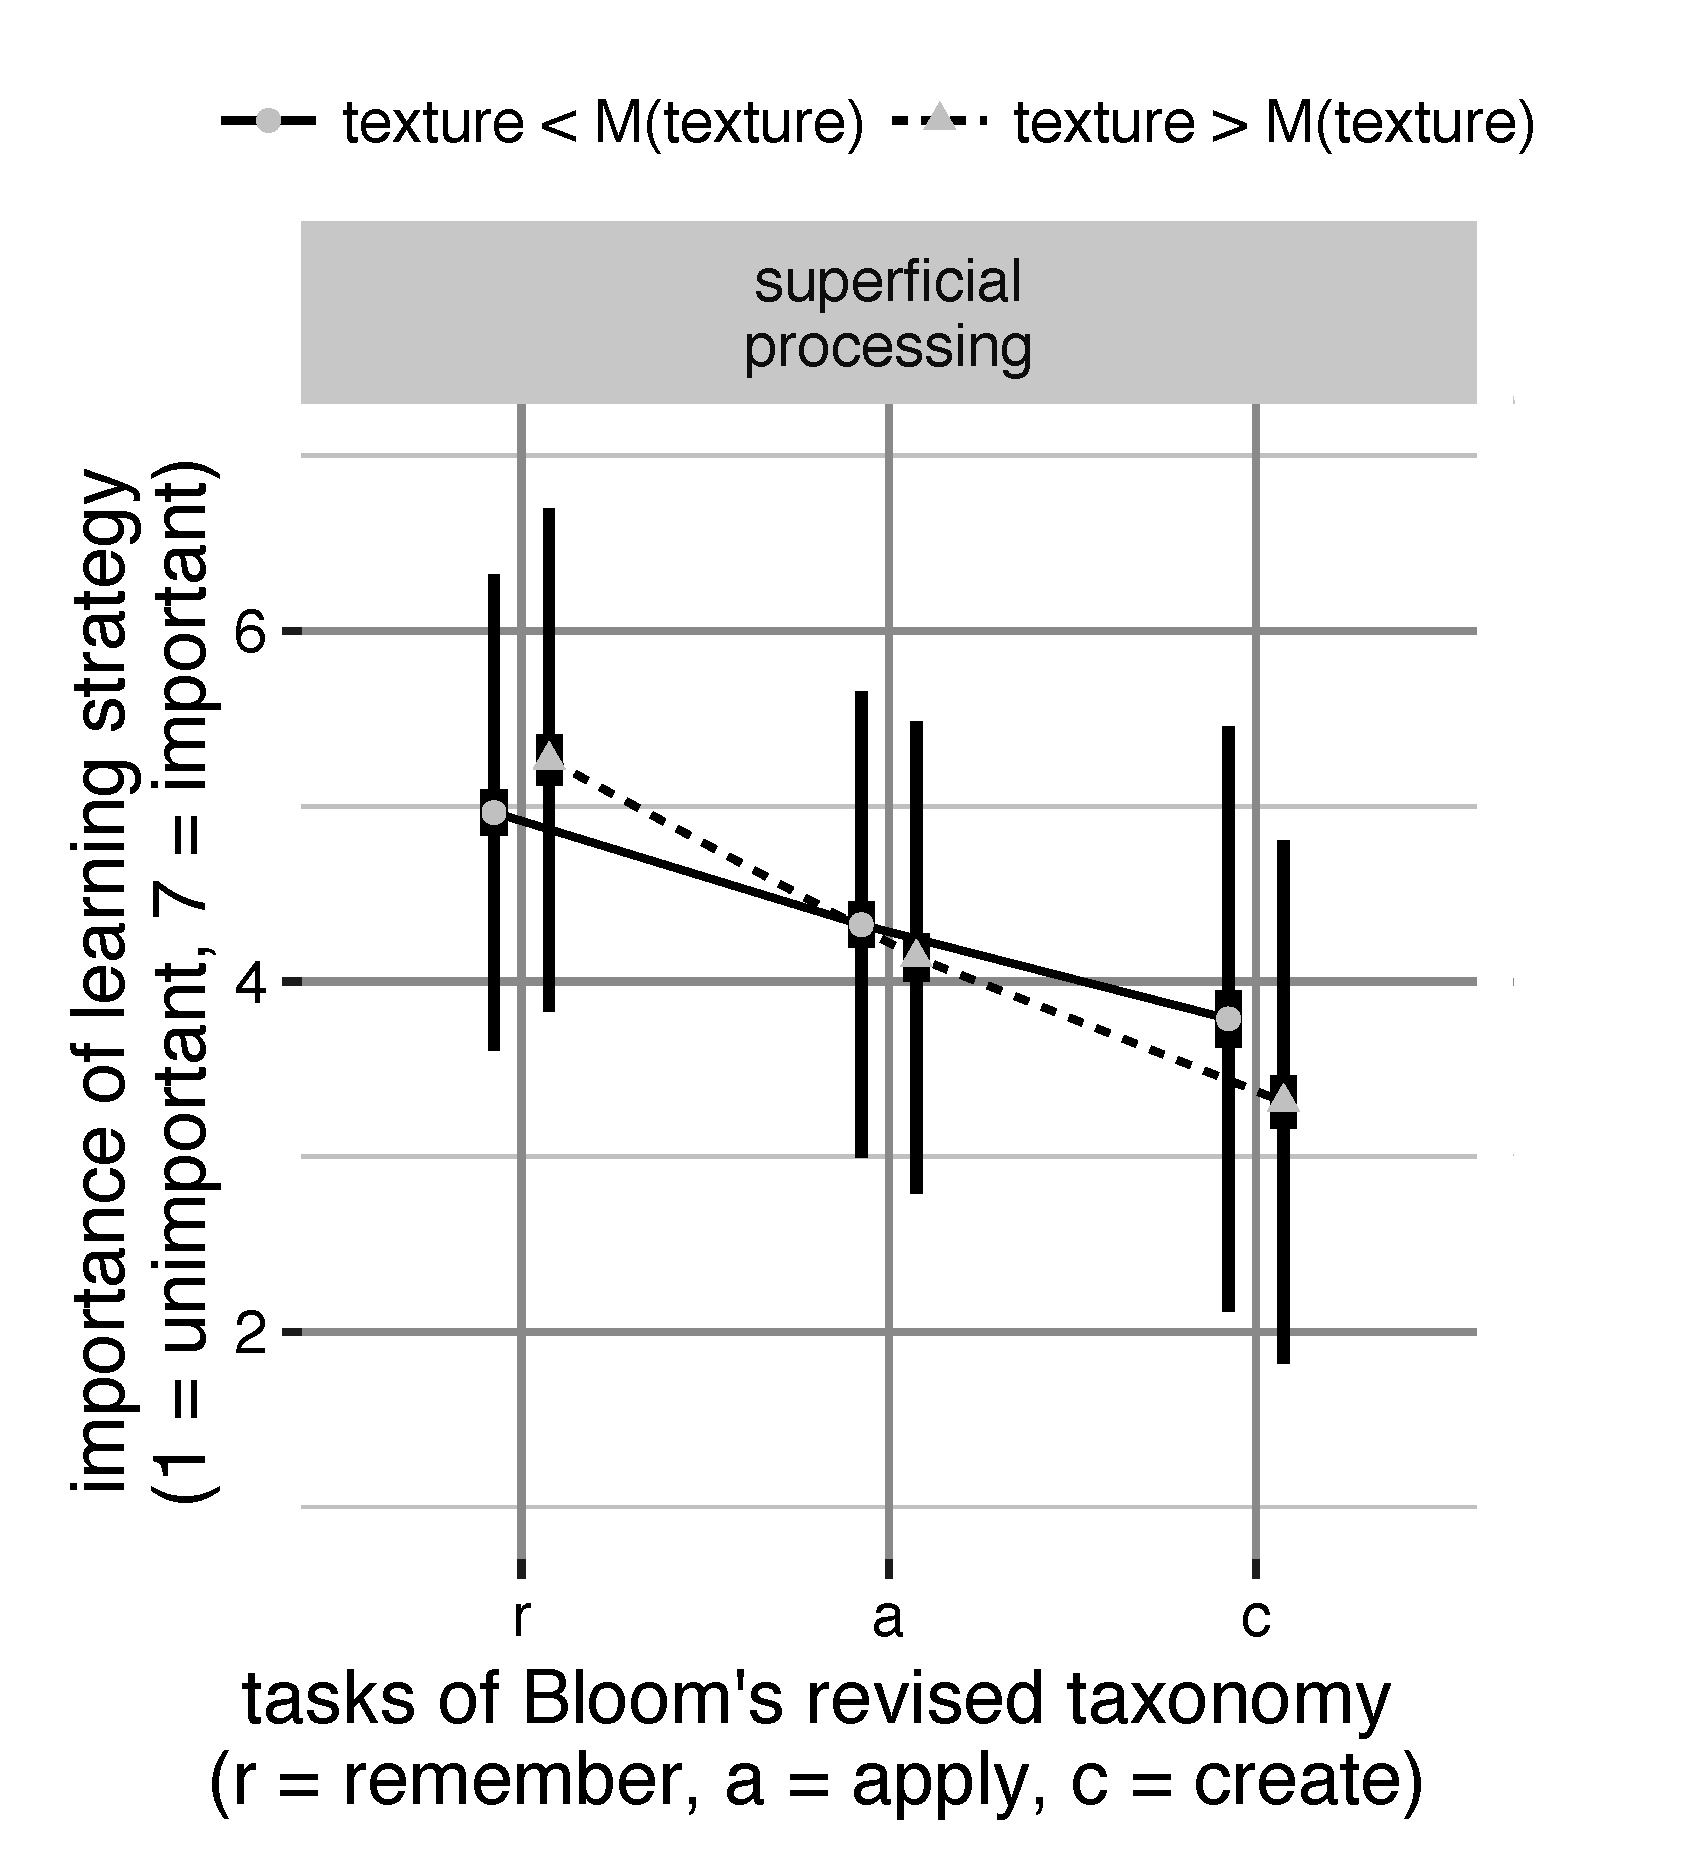
\includegraphics{../Img/Kalibrierung_sup4.png} Lange/kurze vertikale
Linien = \emph{SD}/\emph{CI}, Punkte/Dreicke = \emph{MW}
\end{marginfigure}

\subsection{Epistemische Überzeugungen kalibrieren die
Lernstrategienwahl}\label{epistemische-uberzeugungen-kalibrieren-die-lernstrategienwahl}

Aus dem COPES-Modell selbstregulierten Lernen sind zwei zentrale
Hypothesen zur Rolle epistemischer Überzeugungen diesbezüglich
abgeleitet worden: die Kalibrierungs- und die Konsistenzhypothese. Die
Kalibrierungshypothese nimmt an, dass epistemische Überzeugung- en als
``Linse'' fungieren, welche bspw. die objektive Komplexität von Aufgaben subjektiv
reinterpretiert.

\begin{marginfigure}
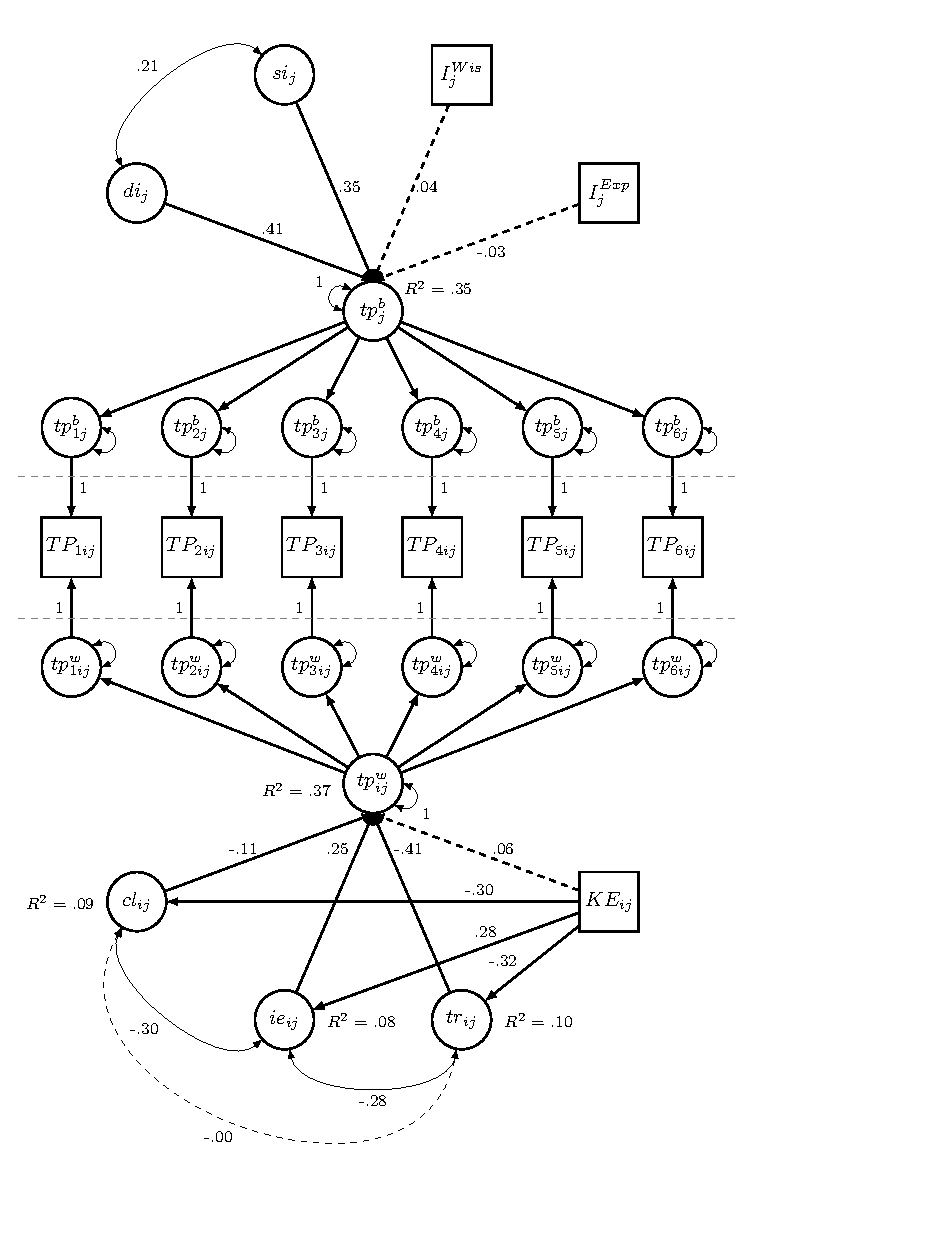
\includegraphics{../Img/mind_the_gap_mlsem.pdf} \(X_{ij}^{w/b}\) =
within-/between-person Wert der Variable X bzgl. Gegenstand i der Person
j, TP/tp = Theorie-Praxis-Integration, di = D-Index (FREE), si =
Studieninteresse, \(I^{Wis/Exp}\) = Indikatorvariable
wissenschaftliche/Experten Quelle, cl = Cognitive Load, ie =
Interest-Enjoy, tr = theorienspezifischer Relativismus, KE = Kenntnis
\end{marginfigure}

\subsection{Epistemische Überzeugungen und
Professionalität}\label{epistemische-uberzeugungen-und-professionalitat}

Epistemische Überzeugungen sind im kompetenztheoretischen Ansatz
generischer Bestandteil von Professionalität im funktionalen Sinne. Im
berufsbiographischen Ansatz können epistemische Überzeugung- en als
notwendige Bedingung für eine angemessene Reflektion der
Bezugswissenschaften gesehen werden. Der Bezug zum strukturtheoretischen
Ansatz ist weit weniger stark. Es konnte in mehreren
Operationalisierungen gezeigt werden, dass die Wahrnehmung
bildungswissenschaftlichen Wissens als sinnvoller Bezugsrahmen für
pä- dagogisches Handeln, auch nach Kontrolle der Quelle des Wissens und
individueller motivationaler Variablen, durch das Entwicklungsniveau
epistemischer Überzeugungen prädiziert wird.

\subsection{Ausblick}\label{ausblick}

Replikationsstudien auf Large-Scale Daten (BILWIS); Epistemische Emotionen, 
epistemische Vertrauenswürdigkeit? Effekte einer
Offenlegung des epistemologischen Status und der Erkenntnismethode
bildungswissenschaftlicher Gegenstände? Epistemische Überzeugungen als
notwendige Bedingung der Professionalitätsentwicklung?

`

\bibliography{../Bib/library.bib}



\end{document}
